\documentclass[12pt]{article}
\usepackage[a4paper, top=0.8in, bottom=0.7in, left=0.8in, right=0.8in]{geometry}
\usepackage{amsmath}
\usepackage{amsfonts}
\usepackage{graphicx}
\usepackage{fancyhdr}
\usepackage{tcolorbox}
\usepackage{enumitem}
\usepackage{setspace}
\usepackage{tikz}
\usepackage[defaultfam,tabular,lining]{montserrat} % Font settings for Montserrat

% General Comment: Template for creating problem sets in a structured format with headers, titles, and sections.
% This document uses Montserrat font and consistent styles for exercises, problems, and performance tasks.

\setlength{\parindent}{0pt}
\pagestyle{fancy}

\setlength{\headheight}{27.11148pt}
\addtolength{\topmargin}{-15.11148pt}

\fancyhf{}
%\fancyhead[L]{\textbf{6.NS.A.1: Dividing Fractions by Fractions - Answer Key}}
\fancyhead[R]{
\includegraphics[width=0.8cm]{Round Logo.png}} % Placeholder for logo
\fancyfoot[C]{\footnotesize © Study Smart Tutors}

\sloppy

%\newcommand{\dfrac}[2]{\frac{#1}{#2}} % New command for display style fractions

\title{}
\date{}
\hyphenpenalty=10000
\exhyphenpenalty=10000

\begin{document}

\subsection*{Problem Set: Dividing Fractions by Fractions - Answer Key}
\onehalfspacing

% Learning Objective Box
\begin{tcolorbox}[colframe=black!40, colback=gray!5, 
coltitle=black, colbacktitle=black!20, fonttitle=\bfseries\Large, 
title=Learning Objective, halign title=center, left=5pt, right=5pt, top=5pt, bottom=15pt]
\textbf{Objective:} Understand how to divide fractions and solve real-world problems involving division of fractions by fractions.
\end{tcolorbox}

% Exercises Box
\begin{tcolorbox}[colframe=black!60, colback=white, 
coltitle=black, colbacktitle=black!15, fonttitle=\bfseries\Large, 
title=Exercises, halign title=center, left=10pt, right=10pt, top=10pt, bottom=60pt]
\begin{enumerate}[itemsep=1em]
    \item Divide: \( \dfrac{2}{3} \div \dfrac{4}{5} \).\\
    \textcolor{red}{\textbf{Solution:} Multiply by the reciprocal: \( \dfrac{2}{3} \times \dfrac{5}{4} = \dfrac{10}{12} = \dfrac{5}{6} \). Answer: \( \dfrac{5}{6} \).}

    \item Simplify: \( \dfrac{5}{6} \div \dfrac{2}{3} \).\\
    \textcolor{red}{\textbf{Solution:} Multiply by the reciprocal: \( \dfrac{5}{6} \times \dfrac{3}{2} = \dfrac{15}{12} = \dfrac{5}{4} \). Answer: \( \dfrac{5}{4} \).}

    \item Solve: \( 3 \div \dfrac{3}{4} \).\\
    \textcolor{red}{\textbf{Solution:} Rewrite as \( 3 \times \dfrac{4}{3} = \dfrac{12}{3} = 4 \). Answer: \( 4 \).}

    \item Divide: \( \dfrac{7}{8} \div 2 \).\\
    \textcolor{red}{\textbf{Solution:} Rewrite as \( \dfrac{7}{8} \times \dfrac{1}{2} = \dfrac{7}{16} \). Answer: \( \dfrac{7}{16} \).}

    \item Divide and simplify: \( \dfrac{4}{9} \div \dfrac{2}{5} \).\\
    \textcolor{red}{\textbf{Solution:} Multiply by the reciprocal: \( \dfrac{4}{9} \times \dfrac{5}{2} = \dfrac{20}{18} = \dfrac{10}{9} \). Answer: \( \dfrac{10}{9} \).}

    \item Write and solve: "A recipe calls for \( \dfrac{3}{4} \) cup of sugar. If this is split equally among \( \dfrac{1}{2} \)-cup portions, how many portions are there?"\\
    \textcolor{red}{\textbf{Solution:} Divide: \( \dfrac{3}{4} \div \dfrac{1}{2} = \dfrac{3}{4} \times \dfrac{2}{1} = \dfrac{6}{4} = \dfrac{3}{2} = 1 \dfrac{1}{2} \). Answer: \( 1 \dfrac{1}{2} \) portions.}

    \item Solve: \( 1 \dfrac{1}{2} \div \dfrac{3}{4} \).\\
    \textcolor{red}{\textbf{Solution:} Convert \( 1 \dfrac{1}{2} \) to \( \dfrac{3}{2} \). Multiply by the reciprocal: \( \dfrac{3}{2} \times \dfrac{4}{3} = \dfrac{12}{6} = 2 \). Answer: \( 2 \).}

    \item Simplify: \( \dfrac{9}{10} \div \dfrac{3}{5} \).\\
    \textcolor{red}{\textbf{Solution:} Multiply by the reciprocal: \( \dfrac{9}{10} \times \dfrac{5}{3} = \dfrac{45}{30} = \dfrac{3}{2} \). Answer: \( \dfrac{3}{2} \).}
\end{enumerate}
\end{tcolorbox}

% Problems Box
\begin{tcolorbox}[colframe=black!60, colback=white, 
coltitle=black, colbacktitle=black!15, fonttitle=\bfseries\Large, 
title=Problems, halign title=center, left=5pt, right=10pt, top=10pt, bottom=10pt]
\textbf{Solve the following problems. Show your work.}

\begin{enumerate}[start=9, itemsep=.5em]
    \item \small A rope is \( \dfrac{5}{6} \) meters long. If it is cut into pieces each \( \dfrac{1}{6} \) meter long, how many pieces are there?  
        {\small \color{red} Solution: Divide \( \dfrac{5}{6} \div \dfrac{1}{6} \). Using the rule for dividing fractions, multiply by the reciprocal:  
        \[
        \dfrac{5}{6} \times \dfrac{6}{1} = \dfrac{30}{6} = 5
        \]
        There are **5 pieces**.}  
      

    \item \small A painter uses \( \dfrac{4}{5} \) gallon of paint for \( \dfrac{1}{4} \) of a wall. How much paint is needed for the whole wall?  
        {\color{red} Solution: Set up the equation \( x = \dfrac{4}{5} \div \dfrac{1}{4} \). Multiply by the reciprocal:  
        \[
        \dfrac{4}{5} \times \dfrac{4}{1} = \dfrac{16}{5} = 3 \dfrac{1}{5}
        \]
        The painter needs **3 \(\dfrac{1}{5}\) gallons** for the whole wall.}  
       

    \item \small A cyclist rides \( 2 \dfrac{1}{2} \) miles every \( \dfrac{3}{4} \) of an hour. How far does the cyclist ride in 1 hour?  
        {\color{red} Solution: Solve \( 2 \dfrac{1}{2} \div \dfrac{3}{4} \). Convert to improper fractions:  
        \[
        \dfrac{5}{2} \times \dfrac{4}{3} = \dfrac{20}{6} = 3 \dfrac{1}{3}
        \]
        The cyclist rides **3 \(\dfrac{1}{3}\) miles per hour**.}  
        {\color{blue} Instructor Note: Encourage students to think of division in terms of "how much per one unit."}

    \item \small Draw a model to represent dividing \( \dfrac{3}{4} \) by \( \dfrac{1}{2} \). Use your model to explain how many groups of \( \dfrac{1}{2} \) fit into \( \dfrac{3}{4} \).  
        {\color{red} Solution: Visually, a fraction strip or area model can show that \( \dfrac{3}{4} \) consists of **one and a half** groups of \( \dfrac{1}{2} \). Algebraically:  
        \[
        \dfrac{3}{4} \div \dfrac{1}{2} = \dfrac{3}{4} \times \dfrac{2}{1} = \dfrac{6}{4} = 1 \dfrac{1}{2}
        \]
        There are **1 \(\dfrac{1}{2}\) groups**.}  
        {\color{blue} Instructor Note: Have students verify their result by multiplying back: \( 1 \dfrac{1}{2} \times \dfrac{1}{2} = \dfrac{3}{4} \).}

\end{enumerate}
        \end{tcolorbox}


\begin{tcolorbox}[colframe=black!60, colback=white, 
coltitle=black, colbacktitle=black!15, fonttitle=\bfseries\Large, 
title=Problems Continued, halign title=center, left=5pt, right=10pt, top=10pt, bottom=10pt]
\textbf{Solve the following problems. Show your work.}


\begin{enumerate}
    \item \small The diagram below shows a total length \( x \) represented as a bar divided into equal sections. Each section is $ \frac{1}{4} $. Write a division equation that represents the diagram and solve for \( x \).

    \begin{center}
    \begin{tikzpicture}
        % Draw the main rectangle
        \draw[thick] (0,0) rectangle (6,1);
        % Divide into six sections
        \foreach \x in {1,2,3,4,5,6} {
            \draw[thick] (\x,0) -- (\x,1);
        }
        % Shade the first five sections
        \foreach \x in {0,1,2,3,4} {
            \fill[gray!30] (\x,0) rectangle (\x+1,1);
        }
        % Label the sections
        \node at (0.5, 0.5) {\( \dfrac{1}{4} \)};
        \node at (1.5, 0.5) {\( \dfrac{1}{4} \)};
        \node at (2.5, 0.5) {\( \dfrac{1}{4} \)};
        \node at (3.5, 0.5) {\( \dfrac{1}{4} \)};
        \node at (4.5, 0.5) {\( \dfrac{1}{4} \)};
    \end{tikzpicture}
    \end{center}

        {\color{red} Solution: The diagram shows 5 sections of \( \dfrac{1}{4} \), so the division equation is:  
       $ 
        x \div \dfrac{1}{4} = 5
        $
                Solving for \( x \), multiply both sides by 4:
    
        $x = 5 \times 4 = 20$
        
        Thus, $ x = 20$.}  
        {\color{blue} Instructor Note: Ask students how the diagram confirms the equation \( x \div \dfrac{1}{4} = 5 \).}

    \item Write and solve: "A piece of fabric is \( 2 \dfrac{1}{3} \) yards long. If each section is \( \dfrac{2}{5} \) yards long, how many sections can be cut?"  
        {\color{red} Solution: Solve \( 2 \dfrac{1}{3} \div \dfrac{2}{5} \). Convert to improper fractions:  
        \[
        \dfrac{7}{3} \div \dfrac{2}{5} = \dfrac{7}{3} \times \dfrac{5}{2} = \dfrac{35}{6} = 5 \dfrac{5}{6}
        \]
        The fabric can be cut into **5 \(\dfrac{5}{6}\) sections**.}  
        {\color{blue} Instructor Note: Have students check by multiplying \( 5 \dfrac{5}{6} \times \dfrac{2}{5} \) to confirm they get the original fabric length.}
\end{enumerate}
\end{tcolorbox}



% Performance Task Box
\begin{tcolorbox}[colframe=black!60, colback=white, 
coltitle=black, colbacktitle=black!15, fonttitle=\bfseries\Large, 
title=Performance Task: Sharing Ingredients, halign title=center, left=10pt, right=10pt, top=10pt, bottom=40pt]
You are preparing for a community bake sale and have the following ingredients:
\begin{itemize}[itemsep=.2em]
    \item \( 6 \dfrac{1}{2} \) pounds of flour.
    \item Each cake requires \( \dfrac{3}{4} \) pound of flour.
    \item Each batch of cookies requires \( \dfrac{2}{5} \) pound of flour.
\end{itemize}
\textbf{Task:}
\begin{enumerate}[itemsep=2em]
    \item Write and solve an equation to find how many cakes can be made. \\
    \textcolor{red}{Solution: Convert total flour: \( 6 \dfrac{1}{2} = \dfrac{13}{2} \).} \\
    \textcolor{red}{Equation: \( \dfrac{13}{2} \div \dfrac{3}{4} \). Multiply by the reciprocal:} \\
    \[
    \textcolor{red}{\dfrac{13}{2} \times \dfrac{4}{3} = \dfrac{52}{6} = \dfrac{26}{3} \approx 8.67 \text{ cakes}.}
    \]
    \textcolor{blue}{Instructor Note: Since we cannot make partial cakes, 8 full cakes can be made.}

    \item Write and solve an equation to find how many batches of cookies can be made. \\
    \textcolor{red}{Equation: \( \dfrac{13}{2} \div \dfrac{2}{5} \). Multiply by the reciprocal:} \\
    \[
    \textcolor{red}{\dfrac{13}{2} \times \dfrac{5}{2} = \dfrac{65}{4} = 16.25 \text{ batches}.}
    \]
    \textcolor{blue}{Instructor Note: Partial batches may not be useful, so only 16 full batches can be made.}

    \item If both cakes and cookies are made, how many pounds of flour will be left? \\
    \textcolor{red}{Flour used for 8 cakes: \( 8 \times \dfrac{3}{4} = \dfrac{24}{4} = 6 \) pounds.} \\
    \textcolor{red}{Flour used for 16 batches of cookies: \( 16 \times \dfrac{2}{5} = \dfrac{32}{5} = 6.4 \) pounds.} \\
    \textcolor{red}{Total flour used: \( 6 + 6.4 = 12.4 \) pounds.} \\
    \textcolor{red}{Flour remaining: \( \dfrac{13}{2} - 12.4 = 0.1 \) pounds (about \( \dfrac{1}{10} \) of a pound).}
    
    \textcolor{blue}{Instructor Note: Discuss whether this leftover amount is enough for another full cake or batch of cookies.}
\end{enumerate}
\end{tcolorbox}

\vspace{1em}
% Reflection Box
\begin{tcolorbox}[colframe=black!60, colback=white, 
coltitle=black, colbacktitle=black!15, fonttitle=\bfseries\Large, 
title=Reflection, halign title=center, left=10pt, right=10pt, top=10pt, bottom=100pt]
What strategies did you use to divide fractions? Reflect on how dividing fractions can be applied to solving real-world problems.

\textcolor{red}{\textbf{Solution:} One common strategy for dividing fractions is to use the "Keep-Change-Flip" method:}
\begin{itemize}
    \item \textcolor{red}{\textbf{Keep:} Keep the first fraction as it is.}
    \item \textcolor{red}{\textbf{Change:} Change the division sign to multiplication.}
    \item \textcolor{red}{\textbf{Flip:} Take the reciprocal (flip) of the second fraction and multiply.}
\end{itemize}
\textcolor{red}{Applying this strategy ensures that fraction division is converted into an easier multiplication problem.}

\textcolor{red}{In real-world applications, dividing fractions is useful when:
\begin{itemize}
    \item \textbf{Cooking:} Adjusting ingredient portions in a recipe.
    \item \textbf{Construction:} Dividing wood or materials into smaller sections.
    \item \textbf{Budgeting:} Splitting expenses evenly among people.
\end{itemize}
}

\textcolor{blue}{\textit{Instructor Note: Encourage students to think of their own examples where fraction division is useful in daily life. Have them explain their reasoning using words and equations.}}
\end{tcolorbox}


\end{document}
